\documentclass[aspectratio=1610]{ctexbeamer}
\usepackage[T1]{fontenc}
\usepackage{mathtools}
\usepackage{tikz}
\usepackage{booktabs}
\usepackage{caption}
\usepackage{outlines}
\usepackage{graphicx}
\usepackage{float}
\usepackage{amsthm}
\usepackage{tabularray}
\usepackage{minted}
\usepackage{hyperref}
\usepackage{underscore}
\usepackage{cleveref}
\RequirePackage{pgfgantt}
\usetheme[
    progressbar=frametitle,
    numbering=fraction,
    subsectionpage=progressbar,
    titleformat title=smallcaps,
    titleformat subtitle=smallcaps,
    titleformat section=smallcaps,
    titleformat frame=smallcaps]{metropolis}

\UseTblrLibrary{booktabs}

\DeclarePairedDelimiter{\set}{\{}{\}}
\DeclarePairedDelimiter{\paren}{(}{)}
\graphicspath{ {./images/} }

\newcounter{fullrefcounter}
\newcommand*{\fullref}[1]{%
\addtocounter{fullrefcounter}{1}%
\label{--ref-\thefullrefcounter}%
\ifthenelse{\equal{\getpagerefnumber{--ref-\thefullrefcounter}}{\getpagerefnumber{#1}}}
  {
    \hyperref[{#1}]{\Cref*{#1} \nameref*{#1}}
  }
  {% false case
    \hyperref[{#1}]{第 \pageref*{#1} 页 \Cref*{#1} \nameref*{#1}}
  }
}
\definecolor{bjutblue}{HTML}{429ABF}
\setbeamercolor{palette primary}{bg=bjutblue}

\setbeamertemplate{footline}{
    \hbox{%
    \begin{beamercolorbox}[wd=\paperwidth,ht=3ex,dp=1.5ex,leftskip=2ex,rightskip=2ex]{page footer}%
        \usebeamerfont{title in head/foot}%
        \hfill
        \begin{tblr}{
            width=.8\linewidth,
            colspec={X[l]X[c]X[r]}
        }
            
        \ifx\insertsubsection\empty
        \else
        \insertsubsection
        \fi
         &
            \ifx\insertsection\empty
            \else
            \insertsection{} 
            \fi
            &
            \insertframenumber{} / \inserttotalframenumber
        \end{tblr}
        \hfill{}
    \end{beamercolorbox}}%
}

\title{Report for Compiler Experiment}
\author{**}
\date{\today}
\ctexset{
    today = small,
    figurename = 图,
    contentsname = 目录,
    tablename = 表,
}

\begin{document}

\maketitle
\begin{frame}{Table of Contents}
    \setbeamertemplate{section in toc}[sections numbered]
    \tableofcontents[hideallsubsections]
\end{frame}

\section{基于递归下降子程序法的三地址代码生成器}
\begin{frame}{主要数据说明}
    \begin{outline}
        \1 Int Lookhead://储存当前lookahead的状态。
            \2 状态包括:NONE, IDN, IF, THEN, ELSE, WHILE, DO, INT10, REAL10, INT8, REAL8, INT16, REAL16, ADD, SUB, MUL, DIV, EQ, GT, LT, LP, RP, SEMI, ASG, WRONG
        \1 String token://储存当前token的值。
        \2 起始符P,非终结符L的结构体
        \1 string code //储存P,L的代码
    \end{outline}
        \begin{columns}
            \begin{column}{0.5\linewidth}
                \begin{outline}
                    \1 非终结符T,F,E的结构体:
                    \2 string code //存放T,E,F的代码
                    \2 string place //存放idn或int或real的值
                \end{outline}
            \end{column}
            \begin{column}{0.5\linewidth}
                \begin{outline}
                    \1 非终结符S的结构体:
                    \2 sstring code //存放S的代码
                    \2 int  begin //S的起始位置
                    \2 int  next //S的下一步的位置
                \end{outline}
            \end{column}
        \end{columns}
    \begin{outline}
        \1 非终结符C的结构体
        \2 string code //存放C的代码
        \2 int  afalse //存放false时跳转位置
        \2 int  atrue //存放true时跳转位置
    \end{outline}
\end{frame}

\begin{frame}[allowframebreaks]{主要函数说明}
    \begin{itemize}
        \item Proc_P: 起始符的子程序,处理P->L,调用L,获取L.code;处理P->LP1,若有用“;”分割的	式子会递归调用自己(P1)。
        \item Proc_L :L的子程序,处理L->S产生式,会调用S并获取S.code;
        \item Proc_S :S的子程序,根据lookhead和结果判断处理的是哪个产生式。
          \begin{itemize}
            \item S->id=E,调用E,获取E.code和E.place并以三地址代码形式写入S.code。
            \item S->if C do S1 (else S2),调用C获得C.code然后递归调用自己(S1)。S1返回后根据			lookhead是不是else决定是否再递归调用S2。最终由C+S1或C+S1+S2生成			自己的S.code。
            \item S->while C do S,调用C然后递归调用自己(S1),由C,S1生成S.code
          \end{itemize}
          \item  Proc_C:先调用E1,获得E1.code,E1.place,然后根据lookhead(是>或<或=)判断处理的是	哪个产生式。不管调用哪个产生式最后只有符号(>,<,=)不一样,都是再调用E2,获得	E2.code,E2.place,然后生成C.code。
          \item   Proc_E:先调用T1,获得T1.code,T1.place,然后根据lookhead(是+或-)判断处理的是哪个	产生式。不管调用哪个产生式最后只有符号(+,-)不一样,都是再调用T2,获得	T2.code,T2.place,然后生成E.code。
          \item   Proc_T:先调用F1,获得F1.code,F1.place,然后根据lookhead(是*或/)判断处理的是哪个	产生式。不管调用哪个产生式最后只有符号(*,/)不一样,都是再调用F2,获得	F2.code,F2.place,然后生成T.code。
          \item   Proc_F:根据lookhead类型判断处理的是哪个产生式。F->idn:F.place = 标识符,F->int/real:F.place = 数值,F->(E),调用E,获得E.place,E.place给F.place,F.place 。
    \end{itemize}
\end{frame}

\begin{frame}{设计思路说明}
    采取的是递归子程序法,分别编写了P,L,S,C,T,F,E的子程序。从P开始深入,每一个子程序都会根据当前的lookhead值来确定当前读到的内容是否符合自己的产生式。
    
    是就会根据对应的产生式去调用其他的子程序,并从中获取其code和place来根据语义规则生成自己的code。并把自己的code返回上级,也就是调用了自己的函数。
    
    最后一层层直到返回到P,P会生成最终的三地址代码,并将其输出。
\end{frame}

\section{基于LR分析法的三地址代码生成器}
\begin{frame}{主要数据结构}
    \begin{outline}
        \1 Sentence类:

        \2 String类型str:存储文法
        \2 Int类型dot:存储文法点的位置
        \3 类函数:addDot:给文法->后添加点
        \2 moveDot:将文法点向后移动一位
        \1 DFA类:
        \2 Vector<string> sentence:存储该状态的文法
        \2 Int num:存储状态的ID
        \2 Int fatherNum:存储能到达该状态的标号(有多个只保留一个)
        \2 Vecotr<int> sonNum:存储该状态能到达的状态标号(不包含自己)
    \end{outline}
    Vector<DFA> LR:存储状态

    Vector<Sentence> input:输入的文法

    r[20][10]:存储分析表的acc和r(+状态号)

    rr[20][10]:存储分析表的状态号

\end{frame}

\begin{frame}{主要函数}
    \begin{outline}
        \1 Init():生成第一个状态S0,把S’->第一个非终结符加入到状态中。
        \1 addSentence(DFA \&dfa):如果->后出现的第一个是非终结符,将该非终结符开始的文法先addDot,然后添加到状态中。
        \1 findSon():从S0开始,给状态S0添加文法。再将每个文法移动dot后的文法作为下个状态。重复这个过程,直到不再有新的状态产生。(每次添加状态前,先判断是否重复)
        \1 状态生成完,先重新编号,再循环一遍找到每个状态的上一个状态和下一个状态。
        \1 Match1(a,b,len):判断状态是不是结束状态,是否是终结文法
        \1 output1(string str):输入非终结符号和终结符号,输出LR表,
    \end{outline}
\end{frame}

\section{基于LLVM的类C语言编译器}

\subsection{Achitecture Design}

\begin{frame}{Architecture Design}
    \begin{outline}
        \1 Use ANTLR4 as lexer and parser generator
            \2 Supports automatic conversion of left-recursive grammars
        \1 Use Rust to write the compiler itself
            \2 Tagged unions
        \1 Use LLVM IR as output
            \2 Produces industrial-quality binaries
            \2 Focus on COMPILER itslef, not on implementation details on target platform
    \end{outline}
\end{frame}

\subsection{Brief introduction of tools used}
\begin{frame}{ANTLR}
    \begin{outline}
        \1 ANTLR: ANother Tool for Language Recognition
        \1 Supports ALL*(Adaptive-LL) grammars
            \2 Produces human-readable code
        \1 Error recovery during lex and parse
        \1 Attirbutes and Actions
        \1 Automatic conversion of lef-recursive grammars
        \1 Even more!
            \2 Semantic predicate
            \2 Customized error recovery
            \2 \dots
    \end{outline}
\end{frame}

\begin{frame}[fragile]{Rust}
    \begin{outline}
        \1 A fairly new language designed by Mozilla
        \1 Tagged Union
        \begin{minted}[breaklines]{rust}
pub enum Type{
    Int(size, signed),
    Pointer(Box<Type> elem),
    ...
}
        \end{minted}
        \1 Safe
            \2 no more segfaults!
    \end{outline}
\end{frame}

\begin{frame}[fragile]{LLVM}
    \begin{columns}
        \begin{column}{0.5\linewidth}
            \begin{outline}
                \1 LLVM
                \1  Focus on compile itself
                    \2 ARCH-VENDOR-OS-ENV
                        \3 x86_64-unknown-linux-gnu
                    \2 Infinate number of registers
                    \2 SSA(Static Signle Assignmend) values
                    \2 Intrinsics
                        \3 Most optimised for target platform
                \1 Large eco-system
                    \2 Clang -- The most modern C compiler
                    \2 Rust
                    \2 Nivdia Cuda Compiler
            \end{outline}
        \end{column}
        \begin{column}{0.5\linewidth}
            \begin{minted}[breaklines=true]{llvm}
# return a + b
define dso_local i32 @add(i32 %0, i32 %1) {
%3 = alloca i32, align 4
%4 = alloca i32, align 4
store i32 %0, i32* %3, align 4
store i32 %1, i32* %4, align 4

%5 = load i32, i32* %3, align 4
%6 = load i32, i32* %4, align 4
%7 = add nsw i32 %5, %6
ret i32 %7
}
            \end{minted}
        \end{column}
    \end{columns}
\end{frame}

\subsection{Language Design}

\begin{frame}{Meet Cb - C, but less}
    \begin{outline}
        \1 Based on ANSI C
        \1 With a bit modification
        \1 \mintinline{c}{int arr[5] -> int[5] arr}
        \1 remove union and enum
        \1 \dots
    \end{outline}
\end{frame}
\begin{frame}{Cb -- Key points}
    \begin{outline}
        \1 Key points
        \pause
        \1 \textbf{Full support of multi-dimentional array}
        \1 \textbf{Full support of structs}
        \1 \textbf{Full support of Pointers}
        \1  Some support of function pointers
        \1 \textbf{And arbitrary combination of types above}
    \end{outline}
\end{frame}
\begin{frame}[fragile, allowframebreaks]{Demo code}
\begin{minted}{c}
int a = 0x1234;
int b = 'a';
char c = 3 + 235;
extern int printf(char*, ...);
char * str = "___Hello world from Cb lang!\n";
struct test{
    int foo;
    char bar;
};
int add(int a, int[] b){
    return a + b[0];
}
int main(int argc, char** argv){
    int[5][2] array;
    int[5]* array_ptr = array;
    struct test ss;
    struct test* ss_pointer = &ss;
    ss.foo = 1234;
    printf(&str[3]);
    printf(str + 3);
    printf("This is %d %d\n", 2 + 1238796, a);
    printf("Argc: %d\n", argc);
    array[0][0] = 0x123;
    printf("array[0][0] = %d\n", array[0][0]);
    printf("array_ptr[0][0] = %d\n", array_ptr[0][0]);
    if(argc == 1) {
        printf("Then\n");
        return -1;
    } else {
        printf("Else\n");
    }
    printf("%d\n", ss.bar);
    {
        int* pointer = &ss.bar;
        *pointer = 0x1234;
        printf("%d\n", ss.bar);
        ss_pointer->foo = 0;
        printf("%d\n", ss.foo);
    }
    printf("A + B = %d\n", add(2, array[0]));
    printf("argv: %s\n", argv[0]);
    1 && printf("not_reached");
    0 && printf("good\n");
    0 || printf("not_reached");
    1 || printf("good\n");
    (0,1) || printf("good\n");
    printf("1+2*3=%d\n", 1 + 2 * 3 * 3 / 3);
    if (!1) {
        printf("not reached");
    } else {
        printf("good\n");
    }
    {
        int i = 0;
        for(i = 0; i < argc; ++ i){
            if (i == 3){
                printf("Break!");
                break;
            } else if(i == 2){
                printf("Contine!");
                continue;
            }
            printf("for %d\n", i);
        }
    }
}

\end{minted}
\end{frame}

\subsection{Lex}
\begin{frame}[fragile]{Lex}
    \begin{outline}
        \1 Use ANTLR as lexer generator
        \1 Optionally prints token stream for debugging
    \end{outline}
    \begin{minted}{text}
        53  'int'                at 1:0
        77  IDENTIFIER           at 1:4
        1   '='                  at 1:6
        78  INTEGER              at 1:8
        3   ';'                  at 1:14
        53  'int'                at 2:0
        77  IDENTIFIER           at 2:4
        1   '='                  at 2:6
        80  CHAR_LITERAL         at 2:8
        3   ';'                  at 2:11
        51  'char'               at 3:0
        77  IDENTIFIER           at 3:5
    \end{minted}
\end{frame}
\subsection{Syntax Analysis and Semantic Analysis}
\begin{frame}[fragile]{Syntax Analysis and Semantic Analysis}
    \begin{outline}
        \1 Do syntax analysis and semantic amalysis in one step
            \2 Thanks to ANTLR
    \end{outline}
\begin{minted}[fontsize=\footnotesize]{text}
addSubExpr
returns[
    Option<Box<dyn ExprNode>> e
]: mulDivExpr {
    $e = $mulDivExpr.e;
} ( '+' mulDivExpr {
    let lhs = (&$e).clone().unwrap();
    let rhs = ($mulDivExpr.e).clone().unwrap();
    let location = $start.start as usize .. recog.get_current_token().stop as usize;
    $e = Some(Box::new(
        report_or_unwrap!(
            BinaryExprNode::new_add(lhs, rhs, location)
            ,recog)
    )  as Box<dyn ExprNode>);
...
\end{minted}
\end{frame}
\begin{frame}{Error reporting}
    All errors discovered during syntax and semantic analysis is reported, and sometimes, recovered.
    \begin{figure}[htp]
      \centering
      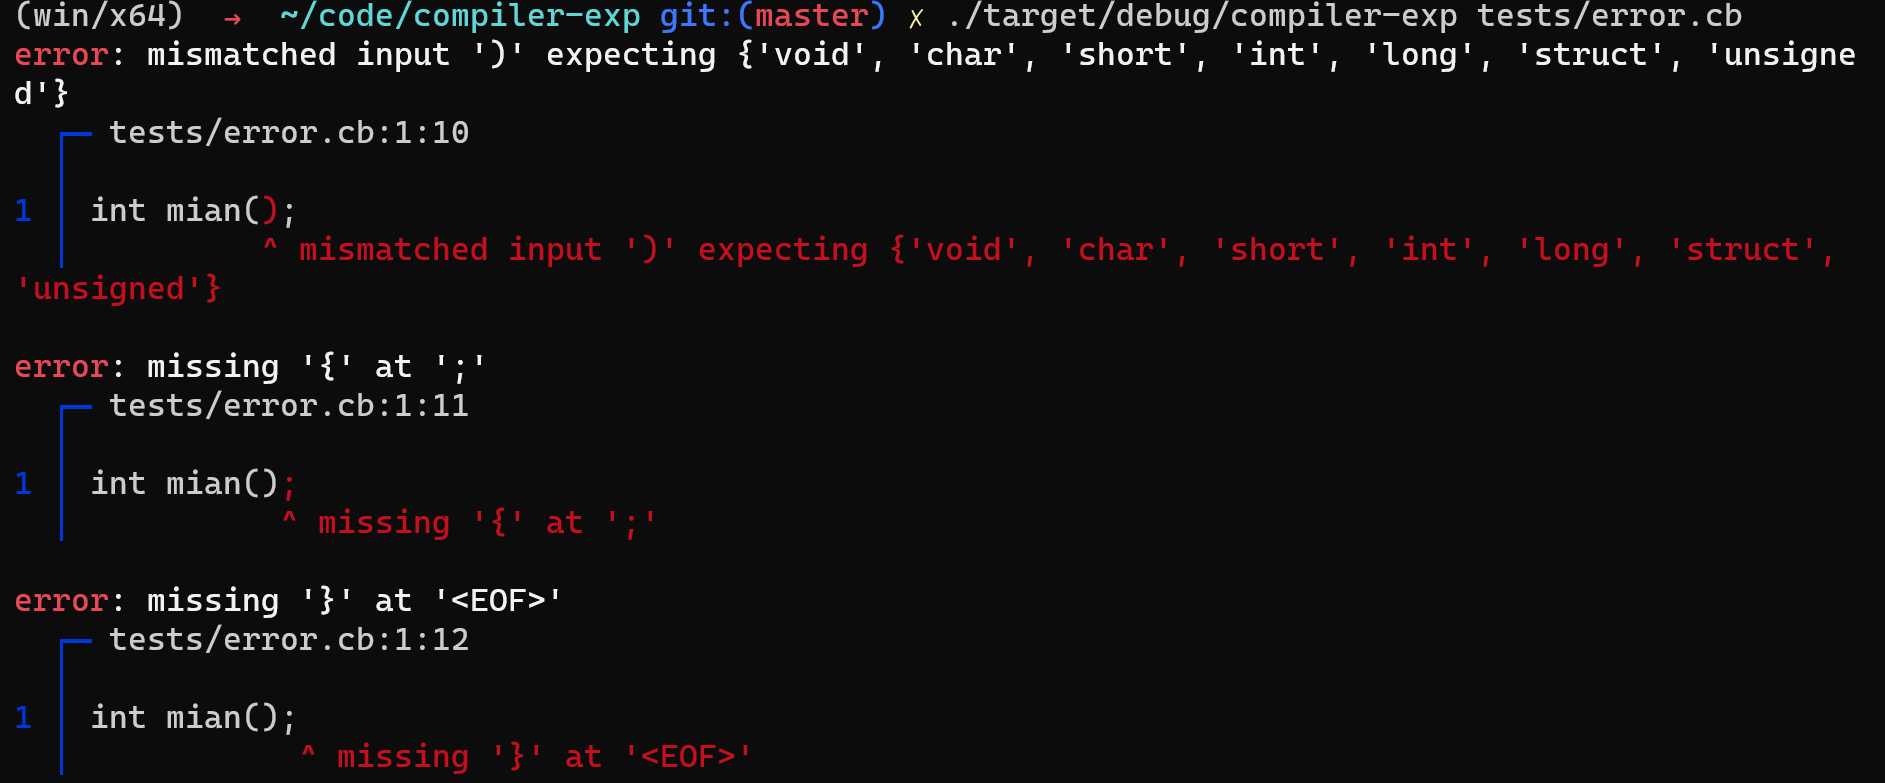
\includegraphics[width=\linewidth]{image1.png}
      \caption{}
    \end{figure}
\end{frame}
\begin{frame}{Error reporting}
    \begin{outline}
        \1 18 types of semantic errors
            \2 TypeNotFound
            \2 VariableNotFound
            \2 EntityNameConflict
            \2 \dots
        \1 All pretty-printed
    \end{outline}
    \begin{columns}
        \begin{column}{.5\linewidth}
            \begin{figure}[htp]
              \centering
              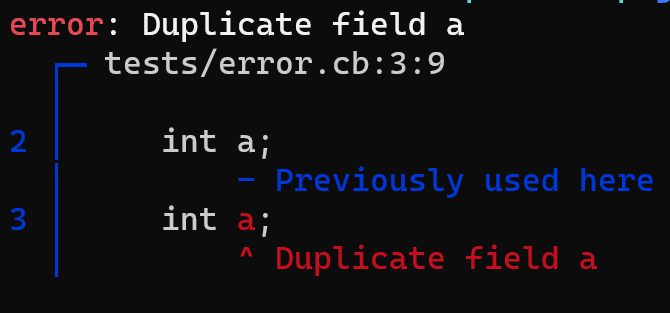
\includegraphics[width=.8\linewidth]{image2.png}
              \caption{}
            \end{figure}
        \end{column}
        \begin{column}{.5\linewidth}
            \begin{figure}[htp]
              \centering
              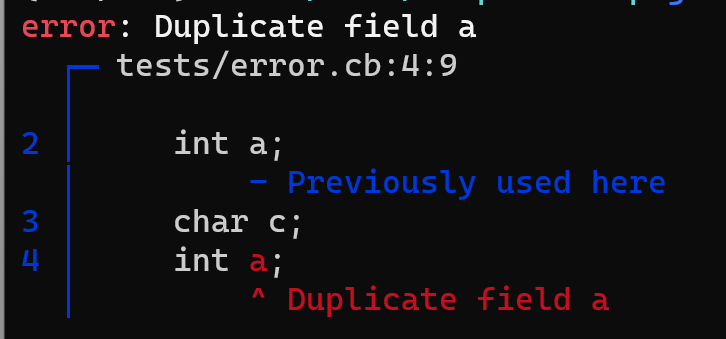
\includegraphics[width=.8\linewidth]{image3.png}
              \caption{}
            \end{figure}
        \end{column}
    \end{columns}
\end{frame}
\begin{frame}[allowframebreaks]{Error reporting}
    \begin{figure}[htp]
      \centering
      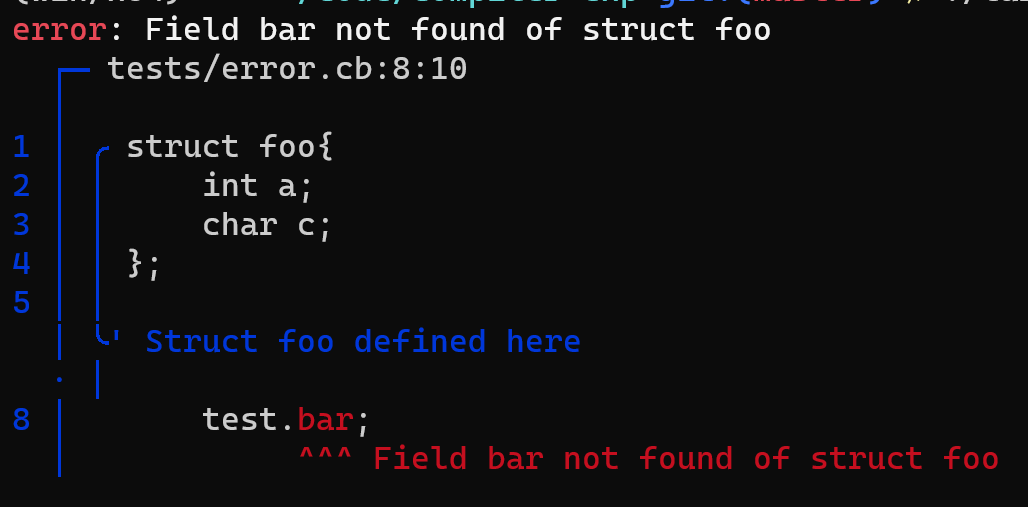
\includegraphics[width=.7\linewidth]{image5.png}
      \caption{}
    \end{figure}
    \begin{figure}[htp]
      \centering
      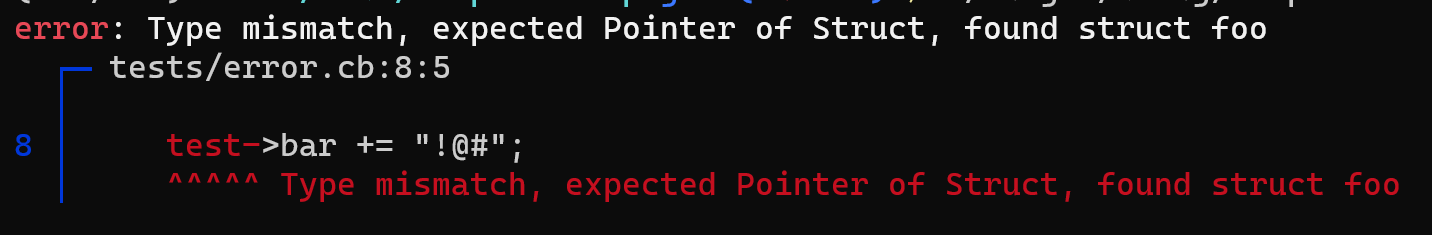
\includegraphics[width=.8\linewidth]{image6.png}
      \caption{}
    \end{figure}
    \begin{figure}[htp]
      \centering
      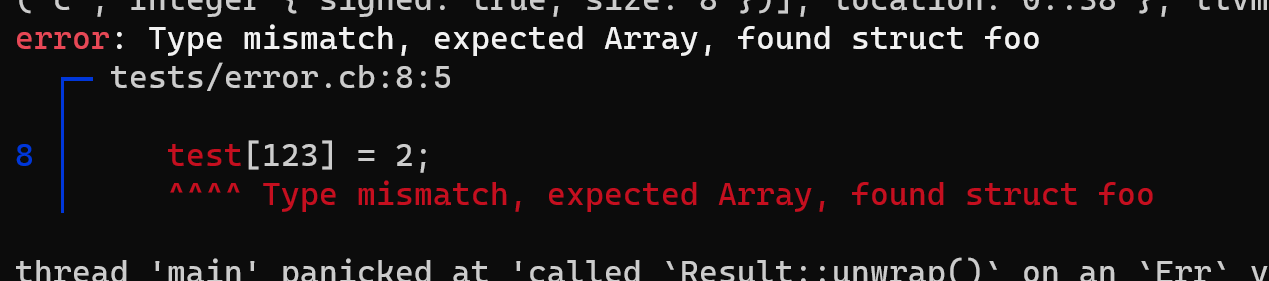
\includegraphics[width=.8\linewidth]{image7.png}
      \caption{}
    \end{figure}
    \begin{figure}[htp]
      \centering
      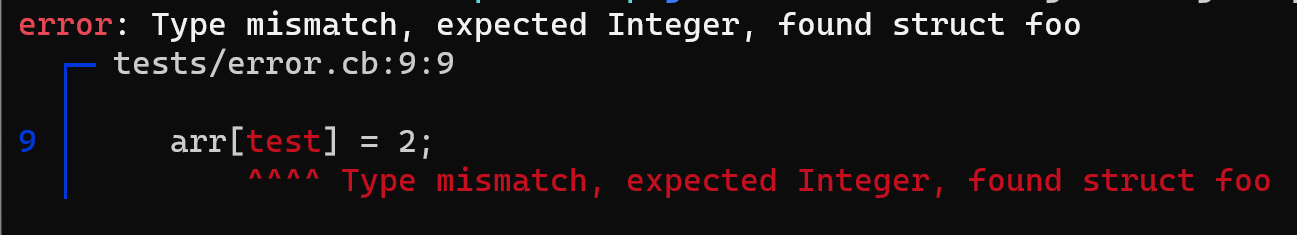
\includegraphics[width=.8\linewidth]{image8.png}
      \caption{}
    \end{figure}
\end{frame}
\subsection{Code generation}
\begin{frame}{Code generation}
    \begin{outline}
        \1 Based on LLVM builder
            \2 another layer of type checking
        \1 Exports LLVM IR for LLVM compiler
    \end{outline}
\end{frame}
\begin{frame}{Code Generation Key Points}
    \begin{outline}
        \1 Support shortcut for logical operators
            \2 \texttt{\&\&} and \texttt{||}
            \2 Uses $\Phi$ node in SSA graph
        \1 Support compile-time constants
            \2 \texttt{int[1+2*3] a;}
    \end{outline}
\end{frame}
\subsection{Limitation}
\begin{frame}{Limitation}
    \begin{outline}
        \1 Incomplete support for function pointers
        \1 No support for recursive types
            \2 Linked Lists
    \end{outline}
\end{frame}
\end{document}
